%%%%%%%%%%%%%%%%%%%%%%%%%%%%%%%%%%%%%%%%%%%%%%%%%%%%%%%%%%%%%%%%%%%%%%%%%%%%%%%%%%
% TEMPLATE INFORMATION:
%%%%%%%%%%%%%%%%%%%%%%%%%%%%%%%%%%%%%%%%%%%%%%%%%%%%%%%%%%%%%%%%%%%%%%%%%%%%%%%%%%
% Stylish Article LaTeX Template - Version 2.1 (1/10/15)
% Downloaded from: http://www.LaTeXTemplates.com
% License: CC BY-NC-SA 3.0 (http://creativecommons.org/licenses/by-nc-sa/3.0/)

%%%%%%%%%%%%%%%%%%%%%%%%%%%%%%%%%%%%%%%%%%%%%%%%%%%%%%%%%%%%%%%%%%%%%%%%%%%%%%%%%%
% TEMPLATE AUTHORS:
%%%%%%%%%%%%%%%%%%%%%%%%%%%%%%%%%%%%%%%%%%%%%%%%%%%%%%%%%%%%%%%%%%%%%%%%%%%%%%%%%%
% ORIGINAL AUTHOR: Mathias Legrand (legrand.mathias@gmail.com) 
% EXTENSIVE MODIFICATIONS: Vel (vel@latextemplates.com)
% FURTHER MODIFICATIONS: Saleem Ameen (saleem.ameen@live.com)
%%%%%%%%%%%%%%%%%%%%%%%%%%%%%%%%%%%%%%%%%%%%%%%%%%%%%%%%%%%%%%%%%%%%%%%%%%%%%%%%%%

%---------------------------------------------------------------------------------
%	PACKAGES AND DOCUMENT CONFIGURATION
%---------------------------------------------------------------------------------

\documentclass[fleqn,10pt]{Stylesheet} % Document font size and equations flushed left
\usepackage[english]{babel} % Specify a different language here - english by default
\usepackage{lipsum} % Required to insert dummy text. To be removed otherwise

%---------------------------------------------------------------------------------
%	COLUMNS
%---------------------------------------------------------------------------------

\setlength{\columnsep}{0.55cm} % Distance between the two columns of text
\setlength{\fboxrule}{0.75pt} % Width of the border around the abstract

%---------------------------------------------------------------------------------
%	COLORS
%---------------------------------------------------------------------------------
\definecolor{color1}{RGB}{139,0,2} % Color of the article title and sections
\definecolor{color2}{RGB}{0,20,20} % Color of the boxes behind the abstract and headings
\definecolor{color3}{RGB}{189,141,29} % Color of the golden lines

%---------------------------------------------------------------------------------
%	HYPERLINKS
%---------------------------------------------------------------------------------

\usepackage{hyperref} % Required for hyperlinks
\hypersetup{hidelinks,colorlinks,breaklinks=true,urlcolor=color2,citecolor=color1,linkcolor=color1,bookmarksopen=false,pdftitle={Title},pdfauthor={Author}}

%---------------------------------------------------------------------------------
%	ARTICLE INFORMATION (E.G. JOURNAL, AUTHORS)
%---------------------------------------------------------------------------------

\JournalInfo{Mars Society, 2020} % Journal information
\Archive{Mars City State Design Competition} % Additional notes
\PaperTitle{Korolev Crater Special Administrative Region} % Article title
\Authors{Alex Sharp\textsuperscript{1}*, Epi Pereria\textsuperscript{2}} % Authors
\affiliation{\textsuperscript{1}\textit{OrionVM}} % Author 1 affiliation
\affiliation{\textsuperscript{2}\textit{Artist}} % Author 2 affiliation
\affiliation{*\textbf{Corresponding author}: alex.sharp@orionvm} % Corresponding author
\Keywords{} % Keywords: Keyword1 --- Keyword2 --- Keyword3
\newcommand{\keywordname}{Keywords} % Defines the keywords heading name

%---------------------------------------------------------------------------------
%	ABSTRACT
%---------------------------------------------------------------------------------
\Abstract{\lipsum[1]~}

%---------------------------------------------------------------------------------
%  START DOCUMENT
%---------------------------------------------------------------------------------

\begin{document}
\flushbottom % Makes all text pages the same height
\maketitle % Print the title and abstract box
\thispagestyle{empty} % Removes page numbering from the first page

%---------------------------------------------------------------------------------
%	INTRODUCTION
%---------------------------------------------------------------------------------

\section*{Introduction} % The \section*{} command stops section numbering
\addcontentsline{toc}{section}{Introduction} % Add to Table of Contents

\lipsum[11] % Dummy text

%---------------------------------------------------------------------------------
%	SECTION 1: TECHNICAL DESIGN
%---------------------------------------------------------------------------------

\section{Technical Design}

For human life to survive, and ultimately, flourish in KCSAR, cost-efficient manufacturing processes of essential bulk materials are critical. This not only ensures economic viability in the presence of high transport costs from Earth, but also mitigates the inherent risk associated with any delays in the transport of critical imports. Given that this requires KCSAR to function within a close to autarkic self-sufficiency framework; this section aims to identify and discuss some of the key technical processes involved in the production of both absolute necessities and utilities, and the productive and intermediary goods that are crucial to the survival and economic development of KCSAR.

\subsection{Absolute Necessities and Utilities}

\subsubsection{Water}
KCSAR is strategically located and built into water ice, which provides readily available access to an abundance of liquid water, provided that the ice is heated. To heat the ice, KCSAR capitalises on the heat exchangers from the reactor designed in section \ref{sec:power_and_thermal_design} that produces a high temperature output that is capable of heating a set of nearby ponds, which dissipate the heat into the surrounding ice walls to ultimately form an inlet of accessible liquid water. While the lake water is not initially potable, a novel two-stage temperature swing solvent extraction (TSSE) process \cite{ChanheeBoo2019}, provides an effective solution. In the first stage, the solvent Diisopropylamine (DIPA) is heated to absorb water from the raw water inlet until it is saturated. This is then cooled so that the DIPA rejects excess water and forms an aqueous layer that can be removed \cite{CRC_84Ed}. In the second stage, Diethyl ether (Eth) is used to extract the DIPA from the water. Given that Eth is mostly immiscible, it is easily removed with a low boiling point and high vapour pressure. Finally, the water is treated to maximise its safety using: (1) activated charcoal filtering, (2) added minerals, (3) NaF for dental health assistance, (4) NaOCl as a disinfectant, and (5) a buffered mixture of common ions to ensure that (a) the pH of the water remains slightly alkaline, (b) metal pipes passivate properly, and (c) leeched metal ions are insoluble.

\subsubsection{Power and Thermal Design}
\label{sec:power_and_thermal_design}

If you are after the priority of life: #0 is energy, and the primary way to make scalable energy, requires a heat sink, which is what the ice is for. 

\subsubsection{Subsubsection}


\subsubsection{Subsubsection}

\subsection{Subsection}

%---------------------------------------------------------------------------------
%	SECTION 2: LIFE ON MARS: SOCIETY AND ECONOMY
%---------------------------------------------------------------------------------

\section{Life on Mars: Society and Economy}

In this section, we lay out the defining characteristics of KCSAR's social and economic makeup. Throughout, we integrate commentary on the ways in which KCSAR's political, cultural and aesthetic makeup contribute to its vibrant society.

\subsection{Governance}

The KCSAR government is made up of four distinct branches, with government powers separated between the executive, legislature, judiciary and an auditor branch. Direct democracy acts as a constraint on the actions political elites, forcing them to represent the interests of the populace at large and to adopt cooperative rather than confrontational strategies. 
\cite{Papadopoulos, 2001}
The KCSAR political system embodies the most direct feasible form of democracy, a delegative democracy. 

Procedural laws substantially limit the powers of each of the branches of government, enforcing substantial oversight from each branch upon the others and requiring that for any substantial change in policy or exercise of non-standard powers, the issue is put to a ranked choice vote by all citizens. Additionally, where matters of judicial interpretation or issues raised by citizens receive a sufficient amount of public support, they are put to a vote. Thereby, citizens directly determine government decisions.

These democratic arrangements are unpopular on Earth primarily because of the prohibitive time cost associated with voting on such a broad range of issues. In KCSAR, this cost is limited through a system of vote delegation by which citizens may delegate their voting right to other individuals or between individuals based on the subject area of the vote. For example, a citizen may delegate their military decisions to person X and economic decisions to person Y. These delegations may be changed at any time and are supported using cryptographic primitives such as homomorphic encryption and linkable ring signatures, allowing for both anonymous voting and cryptographic security.

To incentivize the emergence of delegates and enable them to publicize their voting positions, the government provides a stipend proportionate to the number of votes a delegate receives. Strict campaign financing laws prevent the use of external funds or exercising undue influence to promote a viewpoint. To ensure that decisions are data and logic-led and that a full range of opinions voting options are represented, 'index voters' - robots that vote on specific issues which follow simple 'if then' logical statements or rely on more advanced techniques from machine learning - are employed. The data and logic used in their decision-making is open to the public and auditable.

\subsection{The Malthusian Trap}
The Malthusian Trap emerges where the average individual within an economy produces only as much as they require to live over their life cycle. Modern credit systems reframe the traditional problem by offering emerging economies the ability to finance the 'importation' of a high total factor productivity by utilising capital-intensive productive technologies. The viability the KCSAR economy thus turns on its ability to sustain a high enough economic output to exceed the combined costs of its existing debt burden (interest and loan repayments) and the costs of supporting its citizens. Hence, maintaining a high GDP per capita is the primary concern of KCSAR's emerging economy and its social design prioritises the maximization of GDP per capita, while supporting a more equitable distribution of resources than that found on Earth. Relatively equitable distribution of resources is important not only in ensuring that all citizens are provided for and live a life a without poverty, helping to enhance social stability, but also in generating higher domestic demand and therefore enabling higher productivity gains through economies of scale. \cite{Kogel&Prskawetz, 2000} 

\subsection{Immigration}
Having highly productive citizens is a key priority of KCSAR. High demand to be part of Earth's first extra-planetary colony provided the opportunity to select for ideal candidates using an AI-based actuarial model of a citizen's lifetime production. However, the cost of travelling to KCSAR (USD 500k approx.) continues to make it difficult for otherwise ideal candidates, who are young, well-educated and therefore have limited wealth, to immigrate. The government subsidizes or underwrites a portion of these individuals' ticket prices, enabling them to access commercial loans by reducing the risk to banks of their default. Friends and families of family members are also encouraged to pool collateral to further reduce the risk associated with commercial loans. Thus, government interventions provide the opportunity for Earth's 'best and brightest' to join KCSAR.

\subsection{Fertility}
In the presence of extremely high immigration costs, for an isolated colony to maintain its population, the fertility rate must remain above the replacement rate (approx. 2.1 children per person capable of bearing children). In most developed nations, the fertility rate has been rapidly declining and the direct importation of the culture surrounding fertility in those nations to KCSAR would result in demographic collapse. The incentivization of child-rearing is therefore a first order concern.

\cite{10.1007/s00148-005-0024-0}
\cite{https://www.ncbi.nlm.nih.gov/pmc/articles/PMC3000017/}


In KCSAR, direct economic incentives, such as a Universal Basic Income ('UBI') are offered to guardians proportional to the number of children they care for. Non-cash incentives such as additional leave and guardian allowances are also offered. These incentives are routinely adjusted to maintain a stable fertility rate and help contribute to a culture that celebrates caring for large families while continuing to productively contribute to KCSAR society. 

As the cost of raising children is substantial in both direct costs (such as providing food and atmosphere for the child) and indirect costs (such as the loss of productive labor of parents) KCSAR is concerned with the 'quality' of children - their capacity to contribute to GDP - as well as their quantity. Embryonic selection is used to select for the most fit potential children. Gametes are extracted from parents and fused to form blastocysts. A cell is taken from each blastocyst and its genome is fully sequenced using a nanopore sequencer. The full genome sequence is then processed to generate a polymorphism map that is analysed using artificial intelligence to determine a ‘fitness’ index score. To estimate this fitness function requires the search space be both explored and exploited simultaneously. We use a regret minimising strategy to estimate the value to the population of a particular phenotype and provide this input to an ensemble classifier to best approximate the global maximum of the fitness problem.

The KCSAR also faces a phenotypic diversity bottleneck created by the small size of its population. Studies have shown that a lower limit on a genetic bottleneck is in the tens of thousands, with higher estimates for K selective species like humans that have few offspring but vast resources available for them. As the population must thrive while adapting to the Martian environment, genetic diversity must be thought of as a resource with risk amelioration benefits even for a population as high as one million. Therefore, frozen gametes from screened and compensated individuals are imported to the KCSAR en masse. The transport costs are relatively low due to the light weight of the cargo.

\subsection{Demographics}
To project KCSAR's population demographics, we scale demographics from Gambia, which has a similar fertility rate (3.5 children/woman) and population growth rate (40\%). \cite{https://en.wikipedia.org/wiki/Demographics_of_the_Gambia)} Below, we approximate a demographic pyramid for KCSAR.

\begin{figure}
    \centering
    \includegraphics{}
    \caption{Caption}
    \label{fig:my_label}
\end{figure}

Young children and the elderly are not part of the labor force and are provided for by the government. As the cost of providing for non-productive individuals is much higher on Mars than Earth, the proportion of people who are part of the working population must be relatively high. Assuming various cutoffs for the working age population, we project the occupations of citizens below.

\begin{figure}
    \centering
    \includegraphics{}
    \caption{Caption}
    \label{fig:my_label}
\end{figure}

As is evident from the figures above, the age at which young people enter the workforce has a dramatic impact on the ratio of working age people to others in a society with such a high reproductive rate. While the proportion of the population entering retirement is low, children engaged in schooling are a substantial burden on KCSAR. 

\subsection{Education}
Optimising the educational process and limiting the amount of time spent in education is one of the key methods to increase the working population. With the advent of the information age, ever more efficient educational methodologies have emerged. KSCAR's educational facilities rely on developments in AI-assisted learning such as in optimising curriculum to the needs and abilities of individual students and in adapting examination difficulty to the level of students. Students are grouped together by ability, rather than age group and provided access to pre-recorded lectures, teaching assistants and learning materials from a variety of sources, enabling them to take ownership of maximising the speed of their learning experience. Curricula are simplified and specified to the greatest extent possible so that students are prepared to enter an occupation that reflects both their preferences and ability. Particularly for children, methods that focalize ‘learning through playing’ and student enjoyment are preferred to foster a culture that values and enjoys the process of learning and work.

\subsection{Work}
The majority of the workforce are engaged in key sectors laid out in KCSAR's technical design and the largest proportion are engaged as factory workers. KCSAR does not receive natural sunlight, so rather than relying on traditional day-night shift working cycles, KCSAR workers work to an eight-hour shift cycle that enables continuous work. To maximise the working population proportion, full employment is sustained through a federal jobs guarantee. All able-bodied workers are provided work at below market wages, enabling otherwise unemployed labor for government operations and ventures. The workers are also encouraged to engage in education to reskill and meet the needs of a dynamic labor market.  

\subsection{Retirement}
KCSAR follows the Singaporean model for retirement saving. Each employee pays 10\% of their gross income to purchase stock of the KCSAR Sovereign Wealth Fund (‘KCWF’). The KCWF is a trust, managed by the government, which invests in the equity and debt of local businesses. The value of the KCWF grows at the roughly average rate of the market on KCSAR. On retirement, workers sell down their units to fund a pension. For most workers, this is a sufficient pension but the government contributes to pensions that do not meet a specified living wage cutoff. The sovereign wealth fund receives proceeds from the sale of land, mineral rights, patents generated by public universities and other public goods.

\subsection{System of wages}
All KC citizens receive a Universal Basic Income (‘UBI’), which is a cash payment indexed to the cost of a basket of essential goods and services. The provision of a UBI produces a society in which the basic needs of all citizens are met, which has four primary benefits: 

\begin{enumerate}
    \item On Mars, where space and air have material costs, unemployment and homelessness have even larger social burdens. A UBI provides a security net, helping to tide people over and thereby reducing the number of people who are initially part of cyclical or frictional unemployment from becoming long-term unemployed.
    \item Studies have shown that there is a strong association between relative poverty and crime. In a Mars colony, where crime is relatively difficult and expensive to prosecute, making sure that all individuals have access to a living wage may be a cost-saving measure. 
    \item It provides support to unpaid care workers and individuals who are not engaged in the formal workforce. This in turn relieves pressure on public services that provide care to ill and differently abled people as well as incentivizing the growth of families.  
    \item It simplifies the provision of transfer payments to citizens by eliminating the need for secondary transfer payments. 
\end{enumerate}

The primary objections to a UBI are that it reduces motivation to work and that it perpetuates inequity, as the most wealthy individuals receive the same benefit as the poorest. Incentives to work still exist with a UBI as the receipt of a wage above the UBI award rate is associated with far greater access to luxury goods and particularly preferred foods such as fish and meat. Moreover, a UBI eliminates the structure of adverse incentives that may arise from other social security programs. Traditional social security programs may offer negative net wages for marginal increases in hours worked, whereas the return from work strictly exceeds the additional taxation burden under a UBI system. In KCSAR, the UBI also has a positive net impact on the equitable distribution of income as it is accompanied by a progressive taxation system such that for anyone of middle class or above, the total value of tax paid exceeds the value of the UBI. 

While there is no economy-wide, government mandated ‘minimum wage’ in the KCSAR, unions are formed within each major industry that then demand appropriate working conditions and remuneration for members. In guaranteeing that the returns of corporations are distributed to labor (rather than absorbed entirely by capitalists), labor unions serve an important role in allocating resources to the population most likely to spend them and encourage further growth, as the Marginal Propensity to Consume (‘MPC’) of workers is higher than that of wealthier business owners. These labor unions will operate as delegative institutions. As companies grow larger, the importance of their unions also grows and unions will take on a direct oversight role as members of the company board. 

\subsection{Taxation}
The taxation mix broadly aims to incentivize taxpayers to engage in the most efficient economic activities (maximising GDP per capita) whilst remaining progressive (maintaining a minimum degree of inequitability). The largest component of the taxation mix is a simple income tax, that is highly progressive and ensures that the net effect of the UBI is positive for low income earners but negative for higher ones. Additionally, a substantial inheritance tax will be utilised to reduce wealth inequality and encourage social mobility. Lower wealth inequality is associated with higher capital mobility, as wealth is negatively correlated with MPC and higher social mobility likely improves labor engagement and provides incentives for hard work and innovation

Taxation is also used as a lever to encourage productive economic behaviors. Capital gains taxes are levied on the increased value of capital goods with active asset rollover exemptions that allow for deferral or reduction of tax burden if the profits generated from the sale of a capital asset are reinvested in new capital assets. This will creates an incentive for individuals to reinvest returns, helping to improve liquidity in the capital market and grow the economy as a whole. Land value taxes are levied on the unimproved value of the real estate of the colony (on shops, apartments etc.). This creates an incentive for land to be used for its most efficient purpose and thereby encourages the endogenous formation of regional specialisation. For example, if an area of land were an industrial zone, and it would be more productive for that land to be used for the creation of a shopping area, the tax provides an economic incentive for the industrial zone to relocate, likely to areas that already have a mass of industrial sites, where firms can benefit from the economies of scale of regional specialisation.

\subsection{Property Market}
Within the city of KCSAR, land is granted to private individuals for a fixed duration and may be traded, mortgaged and rented. As each new section of the city is built, the ‘land’ inside is sectioned off for land deeds with a fixed ownership term, which is its design refurbishment lifetime (around 30 to 50 years into the future). On the expiry of the grant, the land is returned to the government, refurbished, redivided and reallocated. This model leads to land growing cheaper over time, making it more accessible to first home buyers. Additionally, mortgages are easily bundled together into collateralized mortgage obligations and are traded between banks, providing a substantial source of liquidity for the short term loan market.

\subsection{Regulation of natural monopolies}
Many of KCSAR's essential markets are natural monopolies in which the cost function of mass production is more highly correlated with the number of distinct designs produced, rather than the number of items that each produces. In particular, regulated modules are the building blocks of the multitude of designs required to service the colony's needs. As these must be produced at scale, through an Original Design Manufacturing model, to minimise costs, they form a natural monopoly. To make these monopolistic industries profitable, while limiting the undue usage of monopoly power, a regulated utility corporation model is used. Candidate organisations are offered monopolitic control over a sector as well as cheap loans provided through the KCWF in exchange for significant public oversight. The charters offered to these organisations issue board seats that are mangaged by the community through delegative democracy. The audit branch is given additional powers to inspect company documents, ensure compliance and to provide the public a means of redress. This oversight also ensures that these corporations are extremely stable, making them ideal candidates for conservative investors.

\subsection{Leased rockets}
An increasingly mature market for leased rockets is pivotal in the reduction of costs associated with interplanetary travel and for the viability of interplanetary trade. A leasing market for reusable rockets enables relatively small companies involved in interplanetary travel and commerce to operate despite extremely high startup costs. As rockets are extremely expensive purchases and proper actuarial models to determine the risk associated with the asset did not yet exist, an insurance policy for the potential shortfall was created to ensure the profitability of investing in rocket ownership. The insurance policy relied on the usage of catastrophe bonds and government intervention through targeted reinsurance programs that restrict the unhedged risk to the insurer to standard commercial risks. This enabled the repackaging and reselling of debt with the same credit rating as the insurer and thereby the on-selling of leases on the wholesale debt market, refilling the initial fund and including extra profit on the lease (a Credit Default Swap). As the market continues to mature and the asset risk is better understood, liquidity continues to improve.

\subsection{Significance and composition of trade}
As an isolated colony, KCSAR remains dependent on key imports from Earth including pharmaceuticals; chemical reagents that are prohibitively expensive or impossible to produce on mars; silicon; and other consumer and capital goods. As the cost of transport is prohibitively high at \$500/kg, these goods are imported in their most weight efficient form. For example, bulk pharmaceuticals are transported as active ingredients and undergo final transformation on Mars. To incentivize importation of capital goods to improve firm productivity, the KCWF is also used to subsidise the import of capital goods. 

To purchase these crucial imports, KCSAR must produce a sufficient quantity of exports. The prohibitive costs of transporting goods to Earth (\$200/kg) requires that only products with extremely high value-add to weight ratios be exported. These products include:

\begin{enumerate}
\item Precious materials are mined from asteroids near Mars by 'Honeybee-style' automated robotic mining. Modelling of the price elasticity of demand or gold, platinum and the like indicate that significant quantities may be exported before oversaturation of supply makes it uneconomical.
\item Fuel mined from comets is exported to refueling stations around the solar system. These stations enable spacecraft that would only able to reach Low Earth Orbit to reach Mars and the outer solar system via an on orbit refueling stage.
\item Creative and productive intellectual property produced on Mars serves as a key export. In particular, on Mars, there is a greater imperative to semi-automate or completely automate tasks, producing a comparative advantage in the creation of some AI systems, designs and datasets. Where applications for efficiency gains in Earth-bound processes are found, these assets are exported with close to zero marginal cost.
\item  The sale of debt and equity will also serve as a key ‘export’ that will finance ventures on Mars, helping to stabilize the balance of trade. In particular capital intensive projects such as mining ventures and infrastructure projects will require external financing which will be recorded as a credit on the capital account.
\item Mars will also has a competitive advantage in the building and operation of telescopes, probes and landers that are to be launched to the far reaches of the solar system. For example, the building of large scale mirrors is far easier on Mars due to its low gravity and access to a vacuum. Some peaks on Mars, such as Olympus Mons also serve as a good location for deep field astronomy.
\item Mars is an ideal candidate for large scale nuclear production, so isotropic extraction from spent fuel will be a significant source of revenue. Nuclear isotopes such as Pu240, Am241 and Co60 are extremely expensive on Earth but would be relatively easy to produce on Mars. Pu240 is used in space probes that are likely to be built nearby in any case.
\item In the future, it’s likely that more uses for zero and low gravity as well as vacuum environments will emerge. It is already clear that some types of research are only possible in these environments. Leasing out space in KC and providing labor to conduct experiment and create these goods may therefore constitute a substantial source of revenue. 

\subsection{The mechanics of trade}

The exchange of packages through the inter-planetary postal services is the basis for trade between KCSAR and earth-bound parties. The KCSAR is a member of the United Postal Union (UPU) and therefore part of the standard postal infrastructure between member states. The distribution network relies on ‘multi-modal’ routing, by which packages are carried by the most cost (or time, depending on the cargo) efficient mixture of trucks, trains, boats, and planes. The final step is a cargo rocket that transports bulk post from Earth to Mars. As Mars is crucially reliant on imports of some necessities, the economic viability of the transportation system that underpins trade is a primary concern.

The results of a sensitivity analysis shown below indicate that the primary mechanism for reducing the transport cost for delivery of freight to Mars is increasing the lifespan and reusability of leased rockets (at least to the 10-year mark). We take the partial derivative of price with respect to a vector of potentially explanatory input variables to provide an indication of how much a change in each factor would impact price. While the rocket lifespan effect dominates, secondary factors such as reducing launch costs (by, for example, connecting the launch complex on Earth to a natural gas pipeline) and reducing the cost of rockets would have significant impact. The technological innovation and reduction in cost of factors of production necessary to change these key factors is most easily stimulated through economies of scale. To enable these economies of scale, a significant market must be generated to enable producers to benefit from scaling up production facilities and investing in research and development.

\begin{figure}
    \centering
    \includegraphics{}
    \caption{Caption}
    \label{fig:my_label}
\end{figure}

Three mechanisms are used to generate stable demand for interplanetary trade: government intervention in its futures market and competition regulation. A futures market for interplanetary trade emerged endogenously, helping to stabilize the demand for and price of traded goods and thereby enabling small and marginal producers to reduce their exposure to liquidity risk and enter the market. It also encouraged more efficient allocation of resources over time. The government intervened by providing a demand floor for interplanetary trade by consistently buying futures for freight transport and using them to transport mail, capital and other government materials. An independent watchdog monitors, reports and provides recommendations to the government on non-competitive behaviors in the rocket production industry. Due to the substantial start-up costs and competitive advantage associated with holding intellectual property in the industry for producing and maintaining rockets. The emergence of vertically integrated firms and firms with substantial market (monopolistic) power is therefore likely. Through the use of the leased rocket model, nonintegrated rocket production companies can easily support an ecosystem of launch providers if they are encouraged to through substantive oversight. A substantially competitive market will keep the costs of production low and encourage innovation amongst competing firms.

\subsection{Culture}
Given that the residents of KCSAR face extraordinary labor and resource scarcity and live in closely contained quarters, it is critical its emerging culture is one that: (a) cultivates a passion for work that is motivated by a desire to advance the collective interests of the colony, (b) values close communal relationships, (c) fosters and applauds innovative thinking, (d) promotes an appreciation and love for both knowledge acquisition, and knowledge sharing, through a life-long pursuit of education, and (e) celebrates large families. 


\cite{https://scholar.smu.edu/cgi/viewcontent.cgi?httpsredir=1&article=1307&context=jalc}
\end{enumerate}


\begin{equation}
\cos^3 \theta =\frac{1}{4}\cos\theta+\frac{3}{4}\cos 3\theta
\label{eq:refname2}
\end{equation}

\lipsum[5] % Dummy text

\begin{enumerate}[noitemsep] % [noitemsep] removes whitespace between the items for a compact look
\item First item in a list
\item Second item in a list
\item Third item in a list
\end{enumerate}

\subsection{Subsection}

\lipsum[6] % Dummy text

\paragraph{Paragraph} \lipsum[7] % Dummy text
\paragraph{Paragraph} \lipsum[8] % Dummy text

\subsection{Subsection}

\lipsum[9] % Dummy text

\begin{figure}[ht]\centering
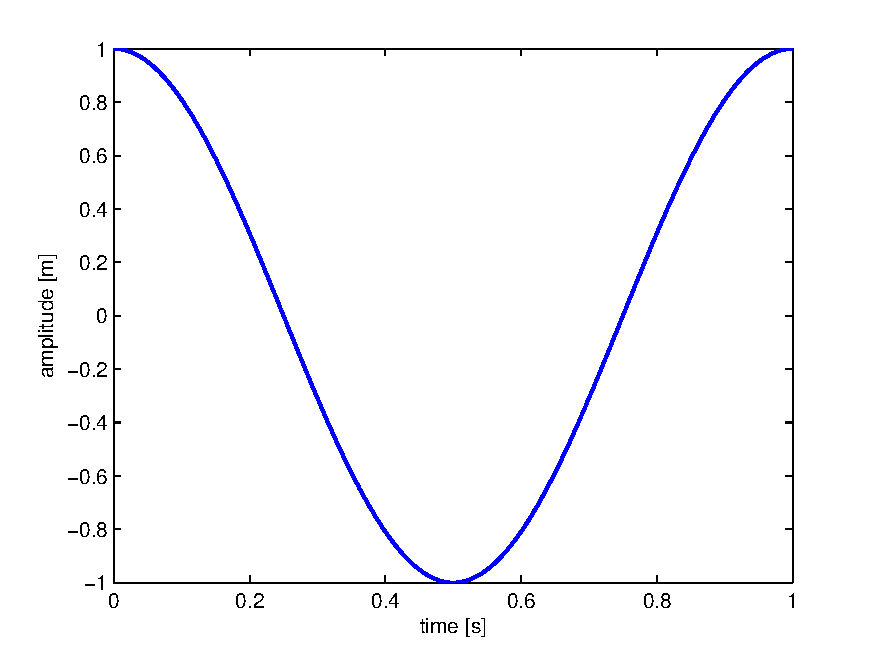
\includegraphics[width=\linewidth]{figures/template_results.pdf}
\caption{In-text Picture}
\label{fig:results}
\end{figure}

Reference to Figure \ref{fig:results}.

%---------------------------------------------------------------------------------
%	SECTION 3: ACKNOWLEDGEMENTS:
%---------------------------------------------------------------------------------
\phantomsection
\section*{Acknowledgments} % The \section*{} command stops section numbering
\addcontentsline{toc}{section}{Acknowledgments} % Add to Table of Contents

So long and thanks for all the fish \cite{Figueredo:2009dg}.

%---------------------------------------------------------------------------------
%	SECTION 4: BIBLIOGRAPHY
%---------------------------------------------------------------------------------
\phantomsection
\bibliographystyle{unsrt}
\bibliography{references}

%---------------------------------------------------------------------------------
%   END DOCUMENT
%---------------------------------------------------------------------------------
\end{document}